\documentclass{article}

% if you need to pass options to natbib, use, e.g.:
% \PassOptionsToPackage{numbers, compress}{natbib}
% before loading nips_2016
%
% to avoid loading the natbib package, add option nonatbib:
% \usepackage[nonatbib]{nips_2016}

\usepackage[final]{nips_2016}

% to compile a camera-ready version, add the [final] option, e.g.:
% \usepackage[final]{nips_2016}

\usepackage[utf8]{inputenc} % allow utf-8 input
\usepackage[T1]{fontenc}    % use 8-bit T1 fonts
\usepackage{hyperref}       % hyperlinks
\usepackage{url}            % simple URL typesetting
\usepackage{booktabs}       % professional-quality tables
\usepackage{amsfonts}       % blackboard math symbols
\usepackage{nicefrac}       % compact symbols for 1/2, etc.
\usepackage{microtype}      % microtypography
\usepackage{graphicx}

\title{Yelp Reviews Topic Modeling to Predict Business Latent Features}

\author{Abby Tisdale \\ Department of Compute Science \\ Harvey Mudd College \\Claremont CA, 91711 \\ atisdale@hmc.edu \And Nicholas Gonzalez \\ Department of Compute Science \\ Harvey Mudd College \\Claremont CA, 91711 \\ ngonzalez@hmc.edu}

% The \author macro works with any number of authors. There are two
% commands used to separate the names and addresses of multiple
% authors: \And and \AND.
%
% Using \And between authors leaves it to LaTeX to determine where to
% break the lines. Using \AND forces a line break at that point. So,
% if LaTeX puts 3 of 4 authors names on the first line, and the last
% on the second line, try using \AND instead of \And before the third
% author name.

  %% examples of more authors
  %% \And
  %% Coauthor \\
  %% Affiliation \\
  %% Address \\
  %% \texttt{email} \\
  %% \AND
  %% Coauthor \\
  %% Affiliation \\
  %% Address \\
  %% \texttt{email} \\
  %% \And
  %% Coauthor \\
  %% Affiliation \\
  %% Address \\
  %% \texttt{email} \\
  %% \And
  %% Coauthor \\
  %% Affiliation \\
  %% Address \\
  %% \texttt{email} \\

\begin{document}

\maketitle

\begin{abstract}
  Yelp has multiple, large, and publicly available datasets.  In this paper we explain research in topic modeling of business reviews which was then used to predict the latent features of businesses.  We began with non-negative matrix factorization for topic modeling of reviews for businesses.  Next we linearly regressed over the topic modeling with each business latent feature to determine if we could predict those latent features.  We also used Multinomial Logistic Regression over the ratings for each business.  Our most notable predictions came from predicting the stars ratings for each business on a 5 point scale.  Our results show promise in the use of topic modeling to predict latent features but also reveal a large amount of work that could be further done to increase accuracy.
\end{abstract}

\section{Introduction}


The Yelp Dataset Challenge provided information about local businesses in 10 cities across 4 countries.  This information includes text reviews, business attributes, check-ins, tips, and photos.  The datasets most relevant to this paper are the business and reviews sets.  The businesses dataset includes over 85,000 businesses with their respective latent features like ?Has TV?, "stars", ?Delivery?, and ?Good for kids?.  The reviews dataset of over 2 million reviews includes the text reviews for each business in the set. 


In order to do topic modeling on the reviews we used non-negative matrix factorization.  Non-negative matrix factorization has been shown to be a useful decomposition for multivariate data.  Our implementation is a variation on an algorithm presented and experimentally tested by Lee and Seung.\footnote{Lee et. al}


We are able to then split the data into training and testing sets.  For each business latent feature which is represented with a binary we linearly regress over the topic modeling data in order to get weights that we can then test on our testing data set.  Similarly for latent features which are over a range, such as stars, we use Multinomial Logistic Regression instead.

Logistic Regression is a common technique for binary categorical classification.  It creates a model based on the probability of a binary classification from a set of independent variables.  This model creates weights that can then be used to predict the binary classification on new data.  Logistic Regression models are prone to over-fitting and overconfidence such that it is not ideal for detecting a small subset which is classified differently.  Despite these limitations, we chose to use this technique because we had many binary classifiers for the businesses such that this technique was easy to apply to each of them individually.  We did however see evidence of over-fitting which was a drawback to using this technique.  The drawbacks were especially evident when a very small subset was classified differently from the majority, as would be expected.

In addition to Logistic Regression we made use of Multinomial Logistic Regression which is an extension to classify within the ratings range.  For instance, the stars rating for a business is on a 5 point scale, so Multinomial Logistic Regression can be used to train a model which given new data can estimate the probability that the new data would be in each of the star categories respectively.  We experimented with different category groupings in efforts to get higher accuracies, but we found that the 5 categories had the best predictions as compared with the probability of random guessing.  The results of those groupings will be discussed more later.

The goal of this experimentation was to determine what, if any, latent features of a business we could predict from its reviews.  The impact of such predictions is obvious in that Yelp or other similar services could predict features without having to procure manual input.  With adequate accuracy, this would allow Yelp to decrease the sparsity of its latent features and provide better service overall.

\section{Procedure}
We started with the set of reviews which were business specific and in individual json objects.  We then collected the reviews for each business into one large review for each business.  We created a frequency list of words for each business, making a sparse matrix.  To decrease the sparse matrix size we also filtered out words that occurred only once and irrelevant high-usage words such as "and" or "the".  At this point we were able to perform the non-negative matrix factorization by minimizing the Frobenius norm between the approximation and the actual matrix.  We also used the multiplicative update for its ease of implementation and guaranteed monotonicity of the objective.\footnote{Dipalo} 


Next we created a matrix of a subset of the latent features for each business.  We chose to filter out any latent features which did not have a true-false value for simplicity.  We then had to reorder the rows of this matrix to match the order of our sparse business-review-topics matrix.  Once we had created our two matrices, one of business and their latent features and the other of businesses and their topic distributions of reviews, we were ready to linearly regress.

After initial investigations with only binary features we also expanded our considerations to include the stars rating for each business.  This involved a very similar process of creating a vector of business ratings so that we could perform Multinomial Logistic Regression.


We split the dataset into a training set of approximately 66\% of the data and and testing set of 33\%.  Then for each latent feature in our subset we linearly regressed with respect to that feature to get appropriate weights.  Next we tested those weights on our testing set so that we could then inspect the accuracy of each prediction to determine which latent features were most easily predicted from review topic modeling. 

For the Multinomial Logistic Regression over ratings we decided to try various groupings in order to discover greater accuracy models.  We considered groupings such as 1-2, 3-4, and 5 as well as 1-3, 4, and 5.  We also tried 1 or 5 compared to 2, 3, or 4.  We realized after the fact that this could have been similarly been done with Logistic Regression since it became a binary.  Our most successful grouping was the standard 5 categories for which the results will be discussed more later.

\section{Challenges}

We had significant troubles trying to work around and overcome the sparsity of the dataset.  Despite having so many businesses and reviews, a surprisingly small subset of businesses had data for the same latent features and often when they did the data was significantly skewed.  For example, a subset of the businesses had the latent feature ?Accepts Credit Cards? but the majority of the businesses with this feature accepted credit cards so our initial attempts at predicting were worse that predicting all businesses would accept credit cards.

Another challenge arose from the copius amounts of useless text in reviews.  In order to determine word frequencies we would have had to consider all of the words in all of the 2 million reviews.  This computation was unreasonable in both space and time considerations.  To work around this computational barrier we had to make sacrifices about how we processed the text reviews.  These sacrifices included dropping single instance words and by using a threshold to leave out overly common words such as "I", "and", or "the".  This allowed topic modeling to be feasible but also limited our dataset.

On top of this we had a difficult time dealing with the amount of fictional or misspelled  words which were in reviews. words such as "Goooood" and "Goood" likely mean the same think however we were not able to register them as the same word. This lead to frequency of words being lower then they should have been as well as greatly increased the number total words which we had to consider. Overall this step of the process was the limiting step in the processing pipeline and caused us to only consider 10,000 business with 400,00 reviews.

Lastly, we faced challenges in trying to predict ratings of businesses.  Although our accuracy for 5 categories was higher than random chance we were disappointed to see even better.  We tried to work around this lower than expected accuracy by trying different groupings but only found our predictions became less useful the more general we made them.

\section{Results}

The first step in our processing pipeline was to generate topics from all of the reviews. The topics generated from reviews are shown in Figure 1.

\begin{figure}
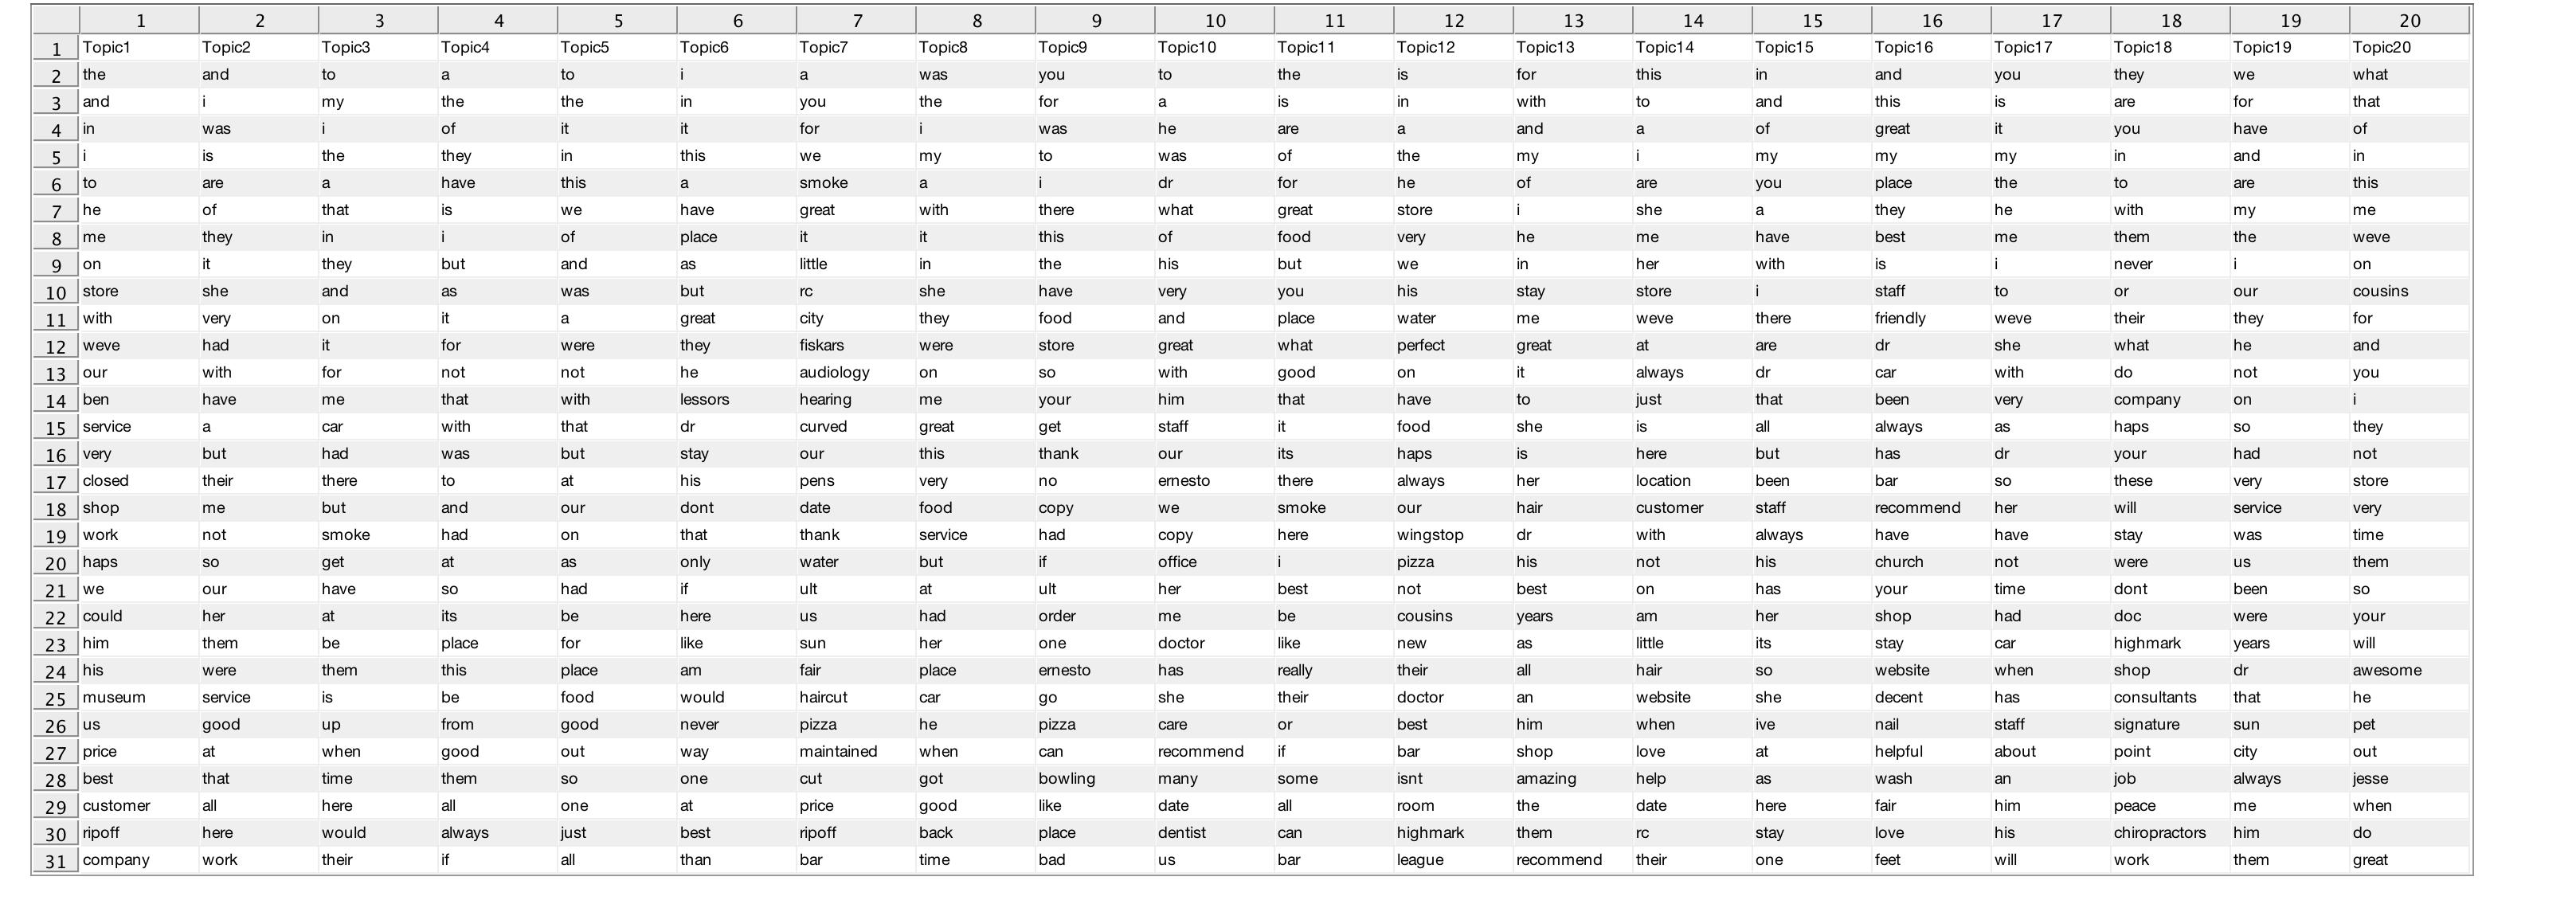
\includegraphics[scale = .13]{topics}
\caption{This figure shows the 20 topics with their top 30 words.}
\end{figure}

The words closest to the top of the column are most important to the topic for their given column.  Upon greater inspection of the topics and the respective words we realized that our thresholds were not quite ideal to filter out words that are not useful such as "I" and "a".

Once the topics were generated we started by using logistic regression to classify whether a business had a particular feature. To do this we simply determined the coefficients using our training set and then classified the testing set by determining if the testing data multiplied by the coefficients was closer to 1 or 0. We ran this individually for each binary latent feature we extracted. The accuracy of each of the classifiers is shown in Figure 2.

\begin{figure}[!h]
\centering
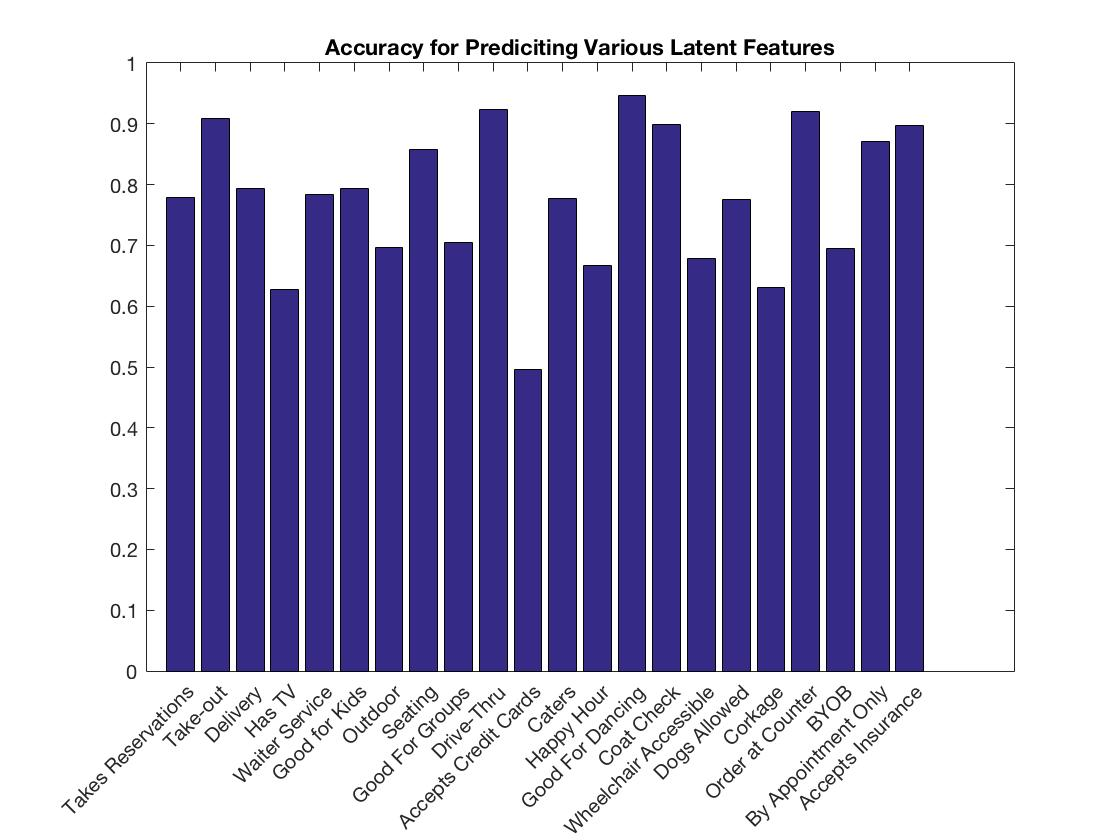
\includegraphics[scale = .3]{fpAccuracy}
\caption{This graph represents the classification accuracy of the classifier for all of the binary latent features we had. As you can see we got an average accuracy of close to 80\%.}
\end{figure}

While these results seemed positive when we looked into our data set closer we notice that in many cases our features had much more of one classification then another. Thus we decided to look into the frequency of false positives and false negatives in our classifications. Our results are shown in figure 3.

\begin{figure}[!h]
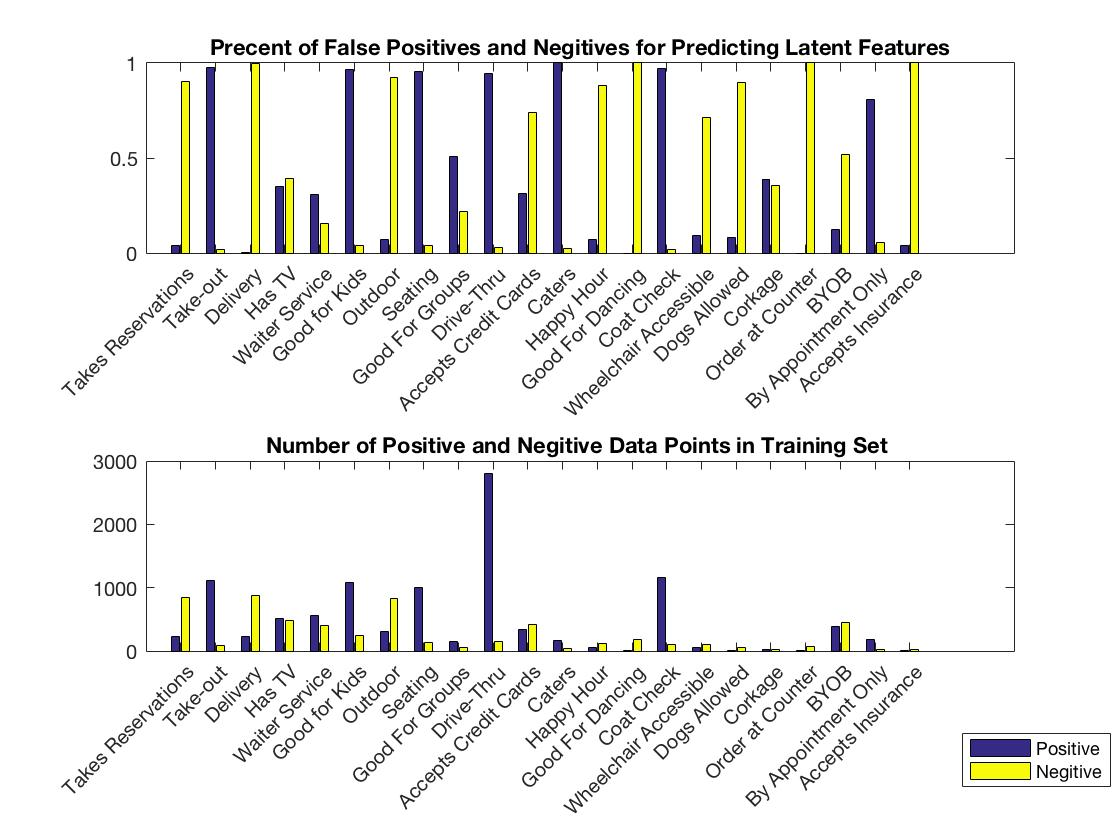
\includegraphics[scale = .3]{fpPlot}
\caption{The top graph shows, for each binary latent feature, the number of each class which was incorrectly classified as a percentage of the total number of this class in the data. The bottom graph shows the number of positive and negative classification in our training set}
\end{figure}

As you can see this clearly  shows that while our classifiers had a high accuracy most were doing a poor job at classifying a particular class. Furthermore we notice that the features which had a high rate of false positives or negatives were  ones where the  classifications were fairly lopsided. We attempted to  reconcile this by over sampling the less likely class but in many cases there were not enough of such classifications to effectively regress on the sample. If we had more time we would expand our data set and look into this approach more closely. One bright note is that in cases of well balanced features such as "Waiter Service" and "Has TV"  our classifier did have both high accuracy, nearly 80\%, and acceptable false negative and false positive errors.

Next we attempted to do ordinal logistic regression to determine the rating of a given business based on their reviews. We ended up using a multinomial logistic regression due to ease of implementation.  The result of this is shown in figure 4 

\begin{figure}[!h]
\centering
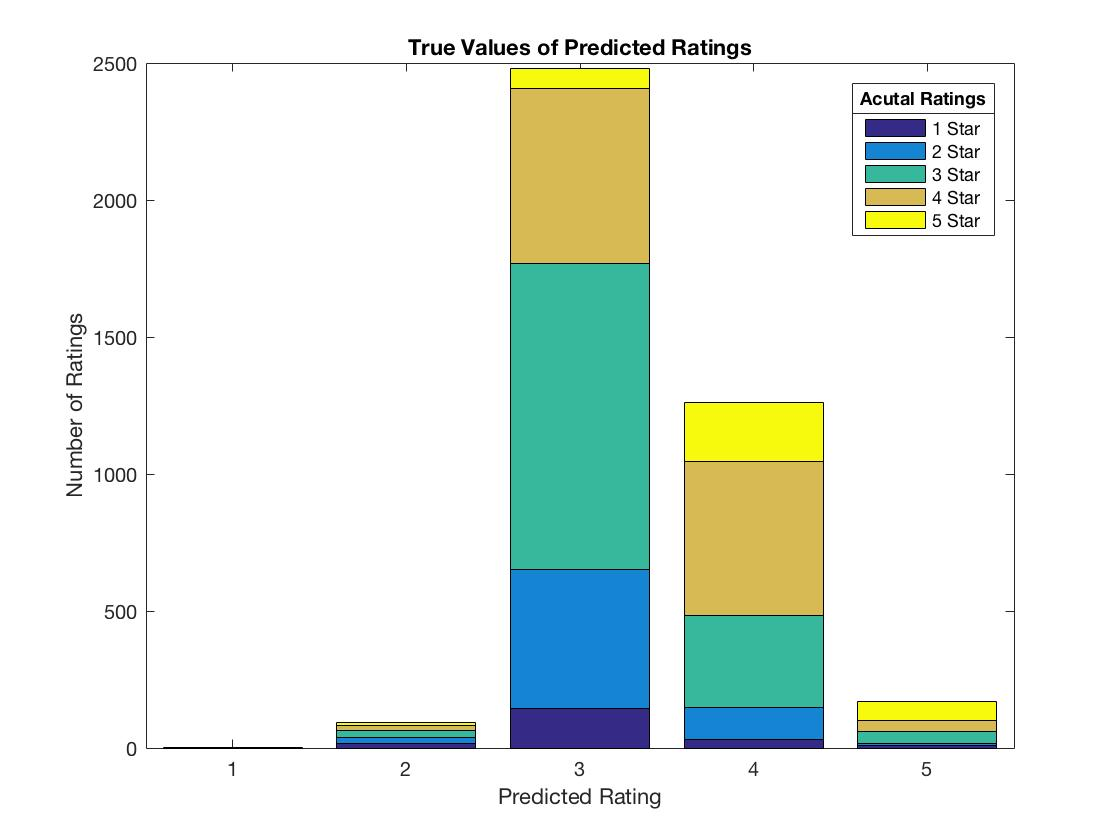
\includegraphics[scale = .4]{../ord}
\caption{This graph shows the classification breakdown when we run the coefficients from our ordinal logistic regression on our training set. The x axis represents the rating as assigned by our classifier while the different colors represent the distribution of actual ratings for each predicted rating. }
\end{figure}

We found that the our classier has a 40\% accuracy which is a significant improvement from the 20\% accuracy from random guessing. Furthermore by looking at the graph it is clear that most of the error is caused from ratings within 1 from the predicted rating, which implies that information about ratings can be observed from the comments.   


\section{Future Work}

Future work could expand the text data sets by finding creative ways to overcome the space and computation restrictions.  This may involve representing the data differently or processing it in unique ways.  Additionally, gaining access to more computing power could simplify many of the problems involved.  There were also other latent features that we did not explore that could be further investigated.

Our most underwhelming results involved latent features for which most businesses either had an entry that was true or did not have an entry at all, such as "Takes Credit Cards".  Our accuracy was severely limited in these features as we were unable to effectively distinguish when a data point should not have been in the category.  Future work could attempt to expand the data set to have more examples for which the feature was false or investigate models which would be more able to distinguish these situations.  One possibility could be to use anomaly detection algorithms and consider elements which are false as anomalies.

Our results of predicting rating from reviews are somewhat trivial and unnecessary since text reviews often accommodate ratings.  However, we see significant potential for using other text sources for which this could be more of an initial proof of concept.  For example, twitter data could potentially be substituted for review text to be the predictor.  Topic modeling as reflected in this paper could be applied to any text repository regarding an entity to then predict ratings.  Thus, future work could investigate the viability of using text inputs other than reviews to predict latent features of businesses or other entities.  

\section*{References}

[1] Lee, Daniel D.\ \& Seung, H. S.\ Algorithms for Non-negative Matrix Factorization, \url{https://papers.nips.cc/paper/1861-algorithms-for-non-negative-matrix-factorization.pdfs}.

[2] DiPaolo, Conner \  (2016) Solution Manual: Math189r Homework 3, Problem 5.

\section*{Links}

Project GitHub: \url{https://github.com/hmc-cs-atisdale/yelp_business_proj}

Yelp Dataset Source: \url{https://www.yelp.com/dataset_challenge/dataset}

\end{document}

